\section{Modellering}
\subsection{Situasjon}
I den første modellen demonstererr vi dempingen som de forskjellig frekvenskomponentene i et signal opplever når det sendes gjennom et medium. Dette gjøres ved å sende et signal med flere frekvenskomponenter gjennom en dempende funksjon, og deretter analysere hvordan de forskjellige komponentene blir påvirket.
Vi tar utgangspunkt i en firkantpuls med periode $T$:
\[
    V_{in}(t) = \begin{cases}
        5, & -\frac{T}{2} \leq t < 0 \\
        0, & 0 \leq t < \frac{T}{2} \\
    \end{cases}, \quad hvor \quad T = 100ns,\qquad duty\ cycle = 50\%
\]
Vi bestemmer først Fourier-rekken til firkantpulsen for å finne frekvenskomponentene:
\[
    V_{in}(t) = \sum_{n=1,3,5,...}^{\infty} c_n e^{j n \omega_0 t}, \quad hvor \quad \omega_0 = \frac{2\pi}{T}
\]
Merk at siden vi vet at duty cycle er 50\%, vil bare oddetalls harmoniske være tilstede i Fourier-rekken.
Koefisientene $c_n$ kan beregnes som:
\[
    c_0 = \frac{1}{T} \int_{-T/2}^{T/2} V(t) dt = \frac{5}{2}
\]
\[
    c_n = \frac{1}{T} \int_{-T/2}^{T/2} V(t) e^{-j n \omega_0 t} dt =  \frac{5}{j 2 n \pi} (1 - (-1)^n)
\]
Vi for dermed at:
\[
    V_{inn}(t) = \frac{5}{2} + \sum_{n=1,3,5,...}^{\infty} \frac{5}{j n \pi} e^{j n \omega_0 t}
\]
For å modellere dempingen i mediet, antar vi en en tilnærment lik realistiske verider for R, G, L og C:
\[
    R(f) = R_{DC} \cdot \sqrt{\frac{f}{f_{s}}}, \quad hvor \quad f_{s} = \frac{\rho_{cu}}{\pi \mu_{cu} r^2}, \quad R_{DC} = n_s \cdot \frac{\rho_{cu}}{\pi r^2}
\]
\[
    \rho_{cu} = 1.72 \cdot 10^{-8} \Omega m, \quad r = 0.255 mm, \quad \mu_{cu} = \mu_0 \cdot \mu_r = 4\pi \cdot 10^{-7} H/m., \quad n_s = 2
\]
\[
    f_s \approx 67kHz, \quad R_{DC} \approx 0.17 \Omega/m,
\]
Dermed får vi:
\[
    R(f) = 0.17 \cdot \sqrt{\frac{f}{67 \cdot 10^3}} \quad [\Omega/m]
\]
Her er $f_s$ den skinneffektsfaktoren for runde ledere, $R_{DC}$ den DC motstanden per meter, $n_s$ tar hensyn til antall lederer i serie (2 for tvinnapar), $\rho_{cu}$ er resistiviteten til kobber, $\mu_{cu}$ er permabiliteten til kobber og $r$ er radiusen til lederen.
Vi antar videre at:
\[
    L = 525 nH/m, \quad C = 52 pF/m
\]
\[
    G(f) = 2\pi f C \tan \delta, \quad hvor \quad \tan \delta = 0.002
\]
Disse verdiene er basert på typiske verdier for en Cat5e kabel og vi står igjen med:
\[
    R(f) \approx 0.17 \cdot \sqrt{\frac{f}{67 \cdot 10^3}} \quad [\Omega/m], \quad L = 525 nH/m, \quad C = 52 pF/m, \quad G(f) \approx 0.65f \quad [pS/m]
\]
\clearpage
\noindent Vi har nå alt vi trenger for å finne overføringsfunksjonen til mediet:
\[
    H(f, l) = e^{-\gamma(f) l}, \quad hvor \quad \gamma(f) = \sqrt{(R(f) + j 2\pi f L)(G(f) + j 2\pi f C)}
\]
Her er $l$ lengden på mediet (kabelen) og $\gamma(f)$ er den komplekse bølgeimpedansen som avhenger av frekvensen.
Vi kan nå finne ut hvordan hver frekvenskomponent i firkantpulsen blir dempet ved å multiplisere hver komponent med $H(f, l)$:
\[
    V_{out}(t) = \sum_{n=1,3,5,...}^{\infty} c_n H(n f_0, l) e^{j n \omega_0 t}
\]
For å simulere dette numerisk, kan vi bruke Python til å beregne $H(f, l)$ for en rekke frekvenser og deretter rekonstruere tidsdomenesignalet ved hjelp av den inverse Fourier-transformasjonen.
Vi kan da plotte både inngangssignalet og utgangssignalet for å visualisere effekten av dempingen i mediet.
\subsection{Modell 1}
Dempinig av signalet over en lengde på 10, 50 og 100 meter er vist i figur \ref{fig:modell1}. Vi ser at høyfrekvente komponenter blir betydelig dempet, noe som resulterer i en mer avrundet firkantpuls ved utgangen. Dette illustrerer hvordan mediet fungerer som et lavpassfilter, hvor de høyere frekvensene reduseres mer enn de lavere frekvensene.
\begin{figure}[h]
    \centering
    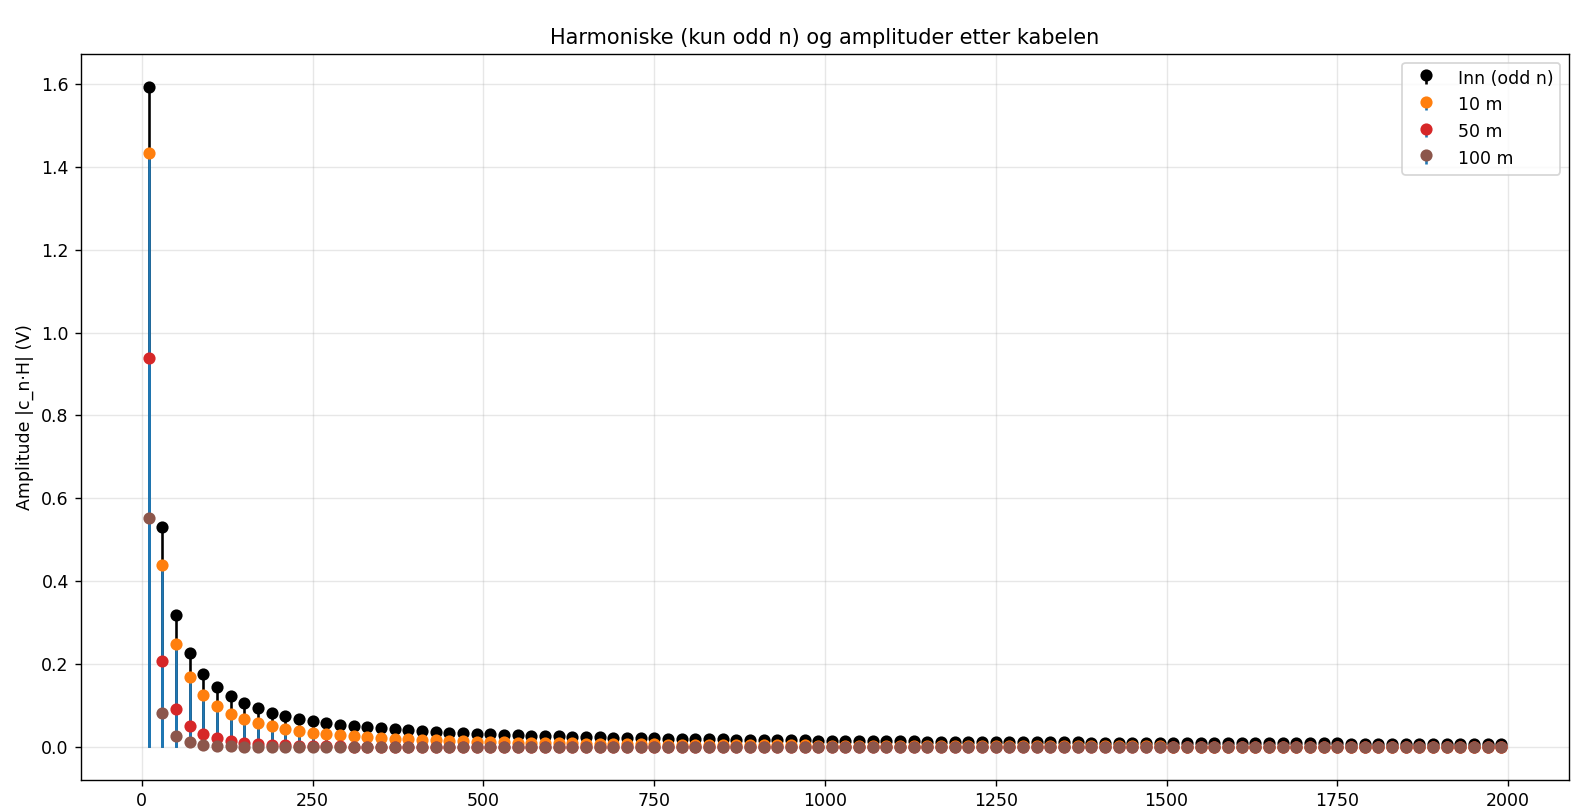
\includegraphics[width=1\textwidth]{Media/modellering1.png}
    \caption{Frekvensdomeneanalyse av firkantpuls etter å ha passert gjennom et dempende medium over forskjellige lengder (10m, 50m, 100m).}
    \label{fig:modell1}
\end{figure}
